\documentclass[10pt,a4paper]{article}
\IfFileExists{spanish.ldf}{\usepackage[spanish,es-tabla]{babel}}{}
\usepackage[utf8]{inputenc}\usepackage[T1]{fontenc}\usepackage{lmodern}
\usepackage[margin=2.25cm]{geometry}
\usepackage{graphicx,booktabs,tabularx,array,amsmath,amssymb,float,caption,xcolor,hyperref,fancyhdr,microtype}
\definecolor{azul}{HTML}{1F5F8B}
\hypersetup{colorlinks=true,linkcolor=azul,urlcolor=azul,citecolor=azul,
  pdftitle={Evaluación Sumativa 1: Análisis exploratorio e inferencial de entregas atrasadas en comercio electrónico},
  pdfauthor={José Ignacio Rodríguez, Yerko Gallardo Miranda, Sebastián Rojas Araya},
  pdfsubject={MCDI501 Estadística Computacional para la Toma de Decisiones, Grupo 1}}
\pagestyle{fancy}\fancyhf{}\lhead{\footnotesize MCDI501 | Sumativa 1}\rhead{\footnotesize Grupo 1}\cfoot{\footnotesize \thepage}
\setlength{\headheight}{14pt}\renewcommand{\headrulewidth}{0pt}
\setlength{\parindent}{0pt}\setlength{\parskip}{4pt}\renewcommand{\arraystretch}{1.12}
\captionsetup{font=small,labelfont=bf,skip=4pt}
\newcommand{\imagen}[4]{\begin{figure}[H]\centering\includegraphics[width=#1\linewidth]{../../outputs/figuras/#2}\caption{#3}\label{#4}\end{figure}}
\newcommand{\codigo}[1]{{\footnotesize\texttt{#1}}}
\renewcommand{\figurename}{Figura}\renewcommand{\tablename}{Tabla}
\begin{document}
\hypersetup{pageanchor=false}\begin{titlepage}\centering\vspace*{1.4cm}
{\large UNIVERSIDAD ANDRÉS BELLO\par}\vspace{.45cm}
{\Large Magíster en Ciencia de Datos e Inteligencia Artificial\par}
\vspace{1cm}{\large MCDI501 Estadística Computacional para la Toma de Decisiones\par}
\vspace{1.3cm}{\Huge\bfseries Evaluación Sumativa 1\par}\vspace{.6cm}
{\LARGE Análisis exploratorio e inferencial de entregas atrasadas en comercio electrónico\par}
\vspace{1.2cm}{\large Grupo 1\par}\vspace{.25cm}
José Ignacio Rodríguez\\Yerko Gallardo Miranda\\Sebastián Rojas Araya
\vspace{1cm}\par Dataset: \emph{E-Commerce Shipping Data}, versión 1\\Octubre de 2026
\vfill\begin{minipage}{.9\linewidth}\small
\textbf{Problema de decisión.} Identificar características y segmentos de envíos que ameriten una investigación operacional posterior. Se caracteriza una base de 10.999 registros, se estiman cuatro parámetros y se presentan siete contrastes con control de multiplicidad. Las asociaciones no permiten atribuir causas ni generalizar automáticamente a una población externa.
\end{minipage}
\vspace{.7cm}\par\small\url{https://github.com/joserodriguezc/grupo_1_estadistica_computacional}
\vspace{.6cm}\par Informe técnico grupal | Ponderación: 20\%
\end{titlepage}\hypersetup{pageanchor=true}

\section{Preparación y carga de datos}
\textbf{Contexto y pregunta.} Según Gopalani (2021), la base reúne envíos de una empresa de comercio electrónico de productos electrónicos. Se pregunta: \emph{¿qué características se asocian con el atraso y qué evidencia orienta una revisión operacional?} La empresa, el período y el marco muestral no están documentados. La unidad provisional es el registro de envío asociado a un cliente; un ID único no garantiza independencia ni un cliente por fila.

El CSV contiene \textbf{10.999 filas y 12 columnas}. Se carga con \codigo{pandas.read\_csv(encoding='utf-8-sig')} y se conserva intacto, con SHA-256 documentado. La copia del repositorio conserva los valores del original de Kaggle. Se crean nombres analíticos y el alias \codigo{entrega\_atrasada}: \textbf{1 = atrasada; 0 = puntual}.
\begin{table}[H]\centering\small
\caption{Clasificación estadística y papel de las doce variables.}\label{tab:diccionario}
\begin{tabularx}{\linewidth}{@{}>{\raggedright\arraybackslash}X>{\raggedright\arraybackslash}X>{\raggedright\arraybackslash}X@{}}\toprule
Variable original & Tipo estadístico & Unidad o categorías\\\midrule
\codigo{ID} & Identificador nominal & Control de unicidad\\
\codigo{Warehouse\_block} & Cualitativa nominal & A, B, C, D, F\\
\codigo{Mode\_of\_Shipment} & Cualitativa nominal & Flight, Road, Ship\\
\codigo{Customer\_care\_calls} & Cuantitativa discreta & Número de llamadas\\
\codigo{Customer\_rating} & Cualitativa ordinal & Escala 1--5\\
\codigo{Cost\_of\_the\_Product} & Cuantitativa de razón & USD, según fuente\\
\codigo{Prior\_purchases} & Cuantitativa discreta & Compras previas\\
\codigo{Product\_importance} & Cualitativa ordinal & low $<$ medium $<$ high\\
\codigo{Gender} & Cualitativa nominal & F, M\\
\codigo{Discount\_offered} & Cuantitativa & Unidad no documentada\\
\codigo{Weight\_in\_gms} & Cuantitativa de razón & Gramos\\
\codigo{Reached.on.Time\_Y.N} & Nominal binaria & 0 puntual; 1 atrasada\\\bottomrule
\end{tabularx}\end{table}

\textbf{Calidad y tratamiento.} Cero nulos, cero duplicados con y sin ID y 10.999 ID distintos; se conservan todas las filas. Los extremos por IQR en compras previas (1.003) y descuento (2.209) se mantienen porque no son errores acreditados. Se verifican dominios, tipos y sumas de frecuencias. No se imputan ni se fabrican faltantes. La bodega F se mantiene pese a que la descripción enumera A--E. El descuento no se interpreta como porcentaje o moneda; ID no se usa en correlaciones.
\imagen{.96}{fig_eda_1_dependiente.pdf}{El atraso afecta al 59,67\% de los registros, frente a 40,33\% puntuales.}{fig:objetivo}
La Figura~\ref{fig:objetivo} muestra 6.563 atrasos y 4.436 puntuales. Dimensiona el problema en el archivo, sin establecer un indicador general del comercio electrónico.


\section{Análisis exploratorio de datos}
\subsection{Centro, dispersión y forma}

\begin{table}[H]
\centering
\scriptsize
\setlength{\tabcolsep}{2.5pt}
\caption{Resumen descriptivo de variables cuantitativas
($n=10\,999$ por variable).}
\label{tab:descriptiva}

\resizebox{\linewidth}{!}{%
\begin{tabular}{@{}lrrrrrrrrrr@{}}
\toprule
Variable & Media & Mediana & DE & Mín. & Q1 & Q3
& Máx. & IQR & A & K \\
\midrule
Llamadas
& 4,05 & 4,00 & 1,14 & 2 & 3,00 & 5,00
& 7 & 2,00 & 0,39 & -0,31 \\

Costo (USD)
& 210,20 & 214,00 & 48,06 & 96 & 169,00 & 251,00
& 310 & 82,00 & -0,16 & -0,97 \\

Compras previas
& 3,57 & 3,00 & 1,52 & 2 & 3,00 & 4,00
& 10 & 1,00 & 1,68 & 4,01 \\

Descuento (u. orig.)
& 13,37 & 7,00 & 16,21 & 1 & 4,00 & 10,00
& 65 & 6,00 & 1,80 & 2,00 \\

Peso (g)
& 3.634,02 & 4.149,00 & 1.635,38 & 1.001
& 1.839,50 & 5.050,00 & 7.846
& 3.210,50 & -0,25 & -1,45 \\

\bottomrule
\end{tabular}%
}
\end{table}

La Tabla~\ref{tab:descriptiva} caracteriza la forma de las distribuciones
con \texttt{stats.skew} y \texttt{stats.kurtosis} de SciPy, con la
opción \texttt{bias=False} en ambas y \texttt{fisher=True} en la curtosis
(SciPy, s.~f.). La curtosis se informa según la definición
de Fisher (curtosis en exceso = curtosis de Pearson $-$ 3),
de modo que una distribución normal tiene asimetría
($A$) y curtosis en exceso ($K$) iguales a cero;
valores positivos de $K$ indican colas más pesadas
que las de una distribución normal.

El peso tiene A = \textbf{\ensuremath{-}0,25} y K = \textbf{\ensuremath{-}1,45}, pero el histograma evidencia bimodalidad. Los coeficientes no prueban normalidad; ni media ni mediana describen por sí solas los dos grupos de valores. El IQR del peso es \textbf{3.210,50 g} y su DE \textbf{1.635,38 g}.
\imagen{.97}{fig_eda_2_cuantitativas.pdf}{Descuento y compras previas presentan colas derechas; el peso tiene dos grupos de concentración. Histogramas y cajas conservan todos los valores.}{fig:cuant}
La Figura~\ref{fig:cuant} respalda la forma de la Tabla~\ref{tab:descriptiva}. Las líneas distinguen media y mediana; no se eliminan extremos. Las llamadas son conteos; calificación e importancia son ordinales y se describen con frecuencias ordenadas, sin distancias iguales entre categorías.


\subsection{Categorías y relaciones bivariadas}
La distribución de las modalidades y demás variables categóricas se presenta en la Figura~\ref{fig:anexo_cualitativas} del Anexo~\ref{sec:anexo_figuras}.

La modalidad marítima (Barco) concentra \textbf{7.462 registros (67,84\%)}, aérea (Avión) 1.777 (16,16\%) y terrestre (Carretera) 1.760 (16,00\%). La bodega F reúne 3.666 registros y cada otra bodega 1.833--1.834. La mediana de calificación es 3 (Q1 = 2; Q3 = 4).
\imagen{.86}{fig_eda_8_dependiente_vs_cualitativas.pdf}{La importancia alta registra 64,98\% de atraso; las diferencias por modalidad y bodega son reducidas. Tasas por categoría con IC individuales de Wilson y n.}{fig:categorias}
En la Figura~\ref{fig:categorias}, importancia alta supera la tasa global de 59,67\%; su V de Cramér frente al resultado es \textbf{0,0333}. Modalidad tiene V = \textbf{0,0082} y bodega V = \textbf{0,0100}. 
Los IC son individuales: que se superpongan o no,
no reemplaza una prueba de hipótesis. La diferencia
de la importancia alta se contrasta formalmente
en E2 y la de modalidad en T01 (sección~4).

\imagen{.58}{fig_eda_5_correlacion.pdf}{Peso y descuento presentan la mayor asociación monótona entre cuantitativas: $\rho=-0{,}316$.}{fig:corr}
La Figura~\ref{fig:corr} usa Spearman para explorar relaciones monótonas mediante rangos. Peso--descuento tiene \textbf{$\rho=-0{,}316$}; llamadas--costo, \textbf{$\rho=0{,}294$}; llamadas--compras previas, \textbf{$\rho=0{,}273$}; costo--compras previas, \textbf{$\rho=0{,}194$}. Las magnitudes bivariadas son limitadas, sin demostrar independencia conjunta ni ausencia de confusión. Se excluyen el identificador, que no tiene significado numérico, y la variable de resultado, cuya relación con cada predictora se analiza por separado en el anexo.


\section{Estimación de parámetros}
Se estiman \textbf{tres medias relevantes y una proporción}. Para la proporción se usa el intervalo de Wilson, recomendado frente al de Wald por su mejor cobertura; para las medias, el intervalo $t$ de Student, $\bar{x}\pm t_{0{,}975;\,n-1}\,s/\sqrt{n}$, con $t_{0{,}975;\,10\,998}=1{,}96018$. Con $n=10\,999$, este coincide con la aproximación normal del TCL ($z_{0{,}975}=1{,}95996$) hasta el segundo decimal, por lo que la elección no afecta los resultados. Wilson se aplica a proporciones, no a medias. Se revisan tamaños, forma, extremos e influencia. Para el resultado binario, $n\hat p=6\,563$ y $n(1-\hat p)=4\,436$. Los intervalos suponen envíos independientes. Este supuesto depende de cómo se obtuvieron los datos y no puede verificarse con estas columnas: no hay identificador de cliente, fecha ni ruta que permita detectar envíos relacionados. Si existiera dependencia (por ejemplo, envíos de un mismo cliente o de una misma carga), los intervalos serían más estrechos de lo que corresponde.

La proporción de atraso es el parámetro central del estudio. Se estiman las medias de peso, costo y llamadas porque tienen unidad documentada e interpretación operacional, y porque peso y costo se comparan entre grupos en T02 y E4. No se estima la media del descuento, cuya unidad no está documentada y cuya fuerte asimetría haría poco representativa la media, ni la de compras previas, conteo asimétrico de baja relevancia para la pregunta.

\begin{table}[H]
\centering
\small
\setlength{\tabcolsep}{4pt}
\caption{Estimaciones e IC individuales del 95\%,
con tamaño muestral y ancho relativo.}
\label{tab:ic}

\begin{tabularx}{\linewidth}{@{}Xrrrrr@{}}
\toprule
Parámetro & n & Estimación & Inferior & Superior
& Ancho rel. (\%) \\
\midrule
Proporción de atraso & 10.999 & 0,59669
& 0,58749 & 0,60582 & 3,07 \\

Peso medio (g) & 10.999 & 3.634,02
& 3.603,45 & 3.664,58 & 1,68 \\

Costo medio (USD) & 10.999 & 210,20
& 209,30 & 211,10 & 0,85 \\

Llamadas medias & 10.999 & 4,054
& 4,033 & 4,076 & 1,05 \\
\bottomrule
\end{tabularx}
\end{table}

Que un intervalo sea de confianza al 95\,\% significa
que el método que lo genera, aplicado a muestras
repetidas, produce intervalos que contienen el
parámetro en aproximadamente el 95\,\% de los casos,
siempre que se cumplan sus supuestos. Ese porcentaje
es una propiedad del método antes de observar los
datos; el intervalo obtenido con esta muestra
contiene o no el parámetro.

La Tabla~\ref{tab:ic} estima un atraso de 59,67\%, con intervalo de Wilson 58,75--60,58\%; peso medio de 3.634,02 g, costo de USD 210,20 y llamadas de 4,054. 
Ningún intervalo supera el 3,1\% del valor estimado,
por lo que todas las estimaciones son precisas. La precisión no corrige selección, dependencia ni incertidumbre del origen. 
Para las proporciones se emplea Wilson al 95\,\%; las tres medias globales, IC $t$ de Student; las diferencias de medias, IC $t$ de Welch, y las diferencias de proporciones, IC de Newcombe. Los intervalos presentados
son individuales, sin ajuste por comparaciones
múltiples.


\section{Pruebas de hipótesis}
Se utiliza $\alpha=0{,}05$ como tolerancia convencional al error tipo I y Holm (1979) para una familia de siete pruebas. Las comparaciones son bilaterales; $\chi^2$ contrasta independencia. Holm no valida umbrales derivados del EDA, como el de descuento mayor que 10 (E3), que es exploratorio.
\subsection{T01 Modalidad y atraso}
$H_0$: modalidad y resultado independientes; $H_1$: asociación. Se emplea \codigo{stats.chi2\_contingency}. Cada envío ocupa una celda y se requiere independencia entre registros.
\begin{table}[H]\centering\small\caption{Frecuencias observadas para el contraste de independencia.}\label{tab:contingencia}
\begin{tabular}{@{}lrrr@{}}\toprule Modalidad & Puntual & Atrasada & Total\\\midrule
Flight & 708 & 1.069 & 1.777\\Road & 725 & 1.035 & 1.760\\Ship & 3.003 & 4.459 & 7.462\\\midrule
Total & 4.436 & 6.563 & 10.999\\\bottomrule\end{tabular}\end{table}
La Tabla~\ref{tab:contingencia} produce $\chi^2(2)=0{,}7434$, $p=0{,}68955$ y V = $0{,}00822$. La mínima frecuencia esperada es 709,82, superior a 5. No se rechaza $H_0$ con Holm; no hay evidencia suficiente de asociación, lo que no demuestra independencia perfecta.


\subsection{T02 Peso medio por resultado}
$H_0:\mu_{atr}-\mu_{punt}=0$; $H_1:\mu_{atr}-\mu_{punt}\ne0$. Welch no impone igualdad de varianzas. Se revisan distribuciones, tamaños e influencia de extremos; independencia y comparabilidad siguen siendo supuestos.

Con \textbf{6.563 atrasadas y 4.436 puntuales}, las medias son \textbf{3.272,64 g y 4.168,67 g}. Diferencia atrasadas menos puntuales: $-896{,}03$ g, IC 95\% $[-956{,}03;-836{,}03]$; $t=-29{,}27$, gl = $9\,526{,}57$ y $p=1{,}93\times10^{-180}$. El efecto $d_{av}=-0{,}569$ divide la diferencia por la raíz de la media de las dos varianzas muestrales. Se rechaza $H_0$ tras Holm, sin inferir causas.
\imagen{.90}{fig_t02_peso_grupos.pdf}{El peso medio es 896,03 g menor entre atrasadas; en (2.000, 4.000] g hay 1.787 atrasadas y una puntual.}{fig:peso}
La Figura~\ref{fig:peso} muestra diferencias de forma; E1 complementa la comparación de medias mediante rangos. 
En el tramo de 2.000 a 4.000 g, 1.787 de los
1.788 envíos llegaron atrasados (99,94\,\%).
Una sola entrega puntual impide que haya
separación completa, es decir, que todos los
envíos del tramo tengan el mismo resultado.
Aun así, en ese tramo el peso predice el
atraso casi sin error, lo que debe considerarse
al modelar el resultado.

\subsection{T03 Descuento medio por resultado}
$H_0:\mu_{atr}-\mu_{punt}=0$; $H_1:\mu_{atr}-\mu_{punt}\ne0$. Welch se utiliza por la diferencia de dispersión: DE = 19,11 en atrasadas y 2,88 en puntuales, con los mismos tamaños de T02.

Las medias son \textbf{18,66 y 5,55 unidades originales}; diferencia $13{,}12$, IC 95\% $[12{,}65;13{,}59]$, $t=54{,}70$, gl = $6\,998{,}09$ y $d_{av}=0{,}960$. La implementación devuelve p = 0 por subdesbordamiento: no es probabilidad matemática nula. Se rechaza $H_0$ tras Holm. El descuento no se expresa como porcentaje ni dinero.
\imagen{.90}{fig_t03_descuento_grupos.pdf}{Ningún envío puntual registra descuento mayor que 10; el segmento comprende 2.647 registros atrasados.}{fig:descuento}
La Figura~\ref{fig:descuento} presenta una separación evidente que
requiere mayor contexto. El dataset no informa
cómo ni cuándo se asigna el descuento; si se
otorgara después del atraso, por ejemplo como
compensación, la relación sería inversa (el
atraso explicaría el descuento) y el descuento
no serviría para predecir atrasos. Aclararlo
requiere documentación de la fuente, no
disponible en estas columnas; por lo tanto,
no se concluye que el descuento cause el atraso.


\subsection{Contrastes complementarios y multiplicidad}
\textbf{E1, rangos del peso.} $H_0$: distribuciones iguales; $H_1$: diferencia detectable por rangos. Mann--Whitney asintótico corrige empates y continuidad: $U=10\,000\,332{,}5$, $p=3{,}40\times10^{-171}$ y efecto biserial de rangos $r=-0{,}313$. Se rechaza $H_0$; sin igualdad de formas no es una prueba exclusiva de medianas.

\textbf{E2, importancia alta.} $H_0:p_{alta}=p_{resto}$; $H_1:p_{alta}\ne p_{resto}$. La prueba z usa proporción combinada bajo $H_0$; los conteos esperados son suficientes. Hay \textbf{64,98\% de atraso en 948 productos de importancia alta}, frente a \textbf{59,17\% en 10.051 del resto}. Diferencia 5,81 puntos porcentuales (pp), IC 95\% de Newcombe [2,57; 8,93] pp; $z=3{,}486$ y $p=0{,}000490$. Se rechaza $H_0$ con Holm, sin identificar causas.

\textbf{E3, descuento mayor que 10.} $H_0:p_{>10}=p_{\le10}$; $H_1:p_{>10}\ne p_{\le10}$. La prueba z combinada tiene conteos esperados bajo $H_0$ mayores que 10: $z=48{,}54$; p no representable como número positivo en la exportación. Se observa \textbf{100\% de atraso en 2.647 registros}, frente a \textbf{46,89\% en 8.352} con descuento $\le10$. Diferencia 53,11 pp; riesgo relativo descriptivo 2,13. El umbral proviene del EDA y exige validación independiente.

El IC de Wilson del grupo > 10 es \textbf{[99,86\%; 100\%]}, no [100\%; 100\%]. El IC 95\% de Newcombe de la diferencia es [52,03; 54,18] pp; al construirse con los intervalos de Wilson de cada grupo, no se degenera cuando un grupo tiene proporción 1, a diferencia del de Wald. No se asume tasa poblacional exactamente igual a 1.


\textbf{E4, costo medio.} $H_0:\mu_{\mathrm{atr}}-\mu_{\mathrm{punt}}=0$; $H_1:\mu_{\mathrm{atr}}-\mu_{\mathrm{punt}}\ne0$. Welch compara USD 207,29 (atrasadas) y USD 214,50 (puntuales); diferencia $-7{,}21$ USD, IC 95\% $[-9{,}03;-5{,}39]$; $t=-7{,}75$, gl = $9\,557{,}16$, $p=1{,}04\times10^{-14}$, y $d_{av}=-0{,}150$. Se rechaza $H_0$ con Holm, pero el efecto es menor que para peso y descuento.
\begin{table}[H]\centering\small\caption{Una familia de siete pruebas, Holm y $\alpha=0{,}05$.}\label{tab:holm}
\begin{tabularx}{\linewidth}{@{}Xlll@{}}\toprule Contraste & p original & p Holm & Decisión\\\midrule
T01 Modalidad & 0,68955 & 0,68955 & No rechazar\\
T02 Peso (Welch) & $1{,}93\cdot10^{-180}$ & $9{,}65\cdot10^{-180}$ & Rechazar\\
T03 Descuento (Welch) & No repr. & No repr. & Rechazar\\
E1 Peso (rangos) & $3{,}40\cdot10^{-171}$ & $1{,}36\cdot10^{-170}$ & Rechazar\\
E2 Importancia alta & 0,000490 & 0,000980 & Rechazar\\
E3 Descuento > 10 & No repr. & No repr. & Rechazar\\
E4 Costo (Welch) & $1{,}04\cdot10^{-14}$ & $3{,}11\cdot10^{-14}$ & Rechazar\\\bottomrule\end{tabularx}\end{table}
``No repr.'' indica subdesbordamiento; se conserva el cero de máquina en CSV sin inventar una cota numérica. La Tabla~\ref{tab:holm} controla multiplicidad de la familia, no vuelve confirmatoria la exploración. No rechazar $H_0$ no demuestra igualdad; significancia no implica importancia operacional.


\section{Interpretación y avance del proyecto}
El atraso de \textbf{59,67\%} justifica investigar el proceso que originó los registros. Modalidad tiene V = \textbf{0,0082} y p Holm = \textbf{0,68955}; no respalda cambiar de transporte. El peso es \textbf{3.272,64 frente a 4.168,67 g}, y descuento \textbf{18,66 frente a 5,55}: asociaciones que requieren explicar composición, temporalidad y registro antes de intervenir sobre carga o política comercial.

\textbf{Recomendación concreta.} Auditar los \textbf{2.647 envíos con descuento > 10}, todos atrasados: verificar cómo se otorgó, si se registró antes o después de la entrega, campañas, productos, fechas, bodegas y rutas. Comparar con los \textbf{8.352 de descuento $\le10$}, cuyo atraso es 46,89\%, y revisar la franja (2.000, 4.000] g. Confirmar el patrón en otro período independiente; el umbral es señal exploratoria, no regla operacional validada.

\textbf{Limitaciones.} Origen muestral y período desconocidos; posible dependencia; confusión no controlada; descuento sin unidad y bodega F discrepante; llamadas y calificaciones potencialmente posteriores al resultado; selección de hipótesis y umbral durante EDA. Ningún p pequeño o IC estrecho elimina estas limitaciones. Los siguientes pasos priorizan procedencia, temporalidad y validación fuera de estos registros.

\section{Notebook y repositorio reproducibles}
\codigo{sumativa\_1/} contiene datos, documentación, notebook, salidas y LaTeX. El notebook se ejecutó en sesión nueva y conserva el SHA-256 del CSV. \codigo{outputs/tablas/entorno\_ejecucion.json} registra Python y versiones utilizadas; \codigo{pyproject.toml} y \codigo{uv.lock} fijan el entorno del equipo. El README detalla rutas y comandos.

\textbf{Procedimientos} (Virtanen et al., 2020; SciPy, s. f.; statsmodels, s. f.):
\begin{itemize}\setlength{\itemsep}{0pt}\setlength{\parskip}{0pt}
\item Carga y controles: \codigo{pandas.read\_csv}, \codigo{isna}, \codigo{duplicated}, \codigo{nunique}, \codigo{crosstab}.
\item Descriptiva y correlación: \codigo{DataFrame.describe}, \codigo{stats.skew}, \codigo{stats.kurtosis},\\ \codigo{DataFrame.corr(method='spearman')}.
\item IC: \codigo{stats.t.ppf} para medias; DE con \codigo{ddof=1}; \codigo{proportion\_confint(method='wilson')} para la proporción global y las tasas por grupo.
\item Contrastes: \codigo{stats.chi2\_contingency}, \codigo{stats.ttest\_ind(equal\_var=False)},\\ \codigo{confidence\_interval(0.95)}, \codigo{stats.mannwhitneyu(method='asymptotic')}.
\item Proporciones: z manual combinado y \codigo{stats.norm.sf}; IC de la diferencia de Newcombe.
\item IC de Newcombe: \codigo{confint\_proportions\_2indep(method='newcomb')}.
\item Holm: \codigo{multipletests(method='holm')}; Cramér: \codigo{stats.contingency.association}.
\end{itemize}
Las tablas proceden de exportaciones, no de imágenes. No se usa simulación ni muestreo aleatorio, por lo que no corresponde semilla. Las salidas pueden regenerarse; la Formativa 1 se conserva como entrega histórica.
\section*{Referencias}\small
Brown, L. D., Cai, T. T., \& DasGupta, A. (2001). Interval estimation for a binomial proportion. \emph{Statistical Science, 16}(2), 101--133.

Cohen, J. (1988). \emph{Statistical power analysis for the behavioral sciences} (2.ª ed.). Lawrence Erlbaum Associates.

Cramér, H. (1946). \emph{Mathematical methods of statistics}. Princeton University Press.

Delacre, M., Lakens, D., Ley, C., Liu, L., \& Leys, C. (2021). \emph{Why Hedges' $g^*_s$ based on the non-pooled standard deviation should be reported with Welch's t-test} [Preprint]. PsyArXiv. \url{https://doi.org/10.31234/osf.io/tu6mp}

Gopalani, P. (2021). \emph{E-Commerce Shipping Data} (versión 1) [Conjunto de datos]. Kaggle. \url{https://www.kaggle.com/datasets/prachi13/customer-analytics}

Holm, S. (1979). A simple sequentially rejective multiple test procedure. \emph{Scandinavian Journal of Statistics, 6}(2), 65--70.

Joanes, D. N., \& Gill, C. A. (1998). Comparing measures of sample skewness and kurtosis. \emph{Journal of the Royal Statistical Society: Series D (The Statistician), 47}(1), 183--189.

Kerby, D. S. (2014). The simple difference formula: An approach to teaching nonparametric correlation. \emph{Comprehensive Psychology, 3}, Artículo 1.

Mann, H. B., \& Whitney, D. R. (1947). On a test of whether one of two random variables is stochastically larger than the other. \emph{The Annals of Mathematical Statistics, 18}(1), 50--60.

Newcombe, R. G. (1998). Interval estimation for the difference between independent proportions: Comparison of eleven methods. \emph{Statistics in Medicine, 17}(8), 873--890.

SciPy. (s. f.). \emph{Statistical functions (scipy.stats)} [Documentación]. \url{https://docs.scipy.org/doc/scipy/reference/stats.html}

Spearman, C. (1904). The proof and measurement of association between two things. \emph{The American Journal of Psychology, 15}(1), 72--101.

statsmodels. (s. f.). \emph{Statistical tests and tools} [Documentación]. \url{https://www.statsmodels.org/stable/stats.html}

Tukey, J. W. (1977). \emph{Exploratory data analysis}. Addison-Wesley.

Virtanen, P., Gommers, R., Oliphant, T. E., Haberland, M., Reddy, T., Cournapeau, D., Burovski, E., Peterson, P., Weckesser, W., Bright, J., van der Walt, S. J., Brett, M., Wilson, J., Millman, K. J., Mayorov, N., Nelson, A. R. J., Jones, E., Kern, R., Larson, E., \ldots{} Vázquez-Baeza, Y. (2020). SciPy 1.0: Fundamental algorithms for scientific computing in Python. \emph{Nature Methods, 17}, 261--272. \url{https://doi.org/10.1038/s41592-019-0686-2}

Welch, B. L. (1947). The generalization of ``Student's'' problem when several different population variances are involved. \emph{Biometrika, 34}(1--2), 28--35.

Wilson, E. B. (1927). Probable inference, the law of succession, and statistical inference. \emph{Journal of the American Statistical Association, 22}(158), 209--212.

\clearpage
\appendix
% Anexos incorporados directamente en este archivo.
% Anexos integrados al documento principal; ruta compartida ../../outputs/figuras/
\begin{center}
{\Large\bfseries Anexos de la Evaluación Sumativa 1}\\[5pt]
{\normalsize Análisis exploratorio e inferencial de entregas atrasadas}\\[4pt]
{\small Grupo 1 --- MCDI501 --- Octubre de 2026}
\end{center}
\noindent\textit{Documento complementario al informe principal. Las figuras siguientes no se reproducen en el cuerpo del informe; los resultados y las limitaciones se interpretan sin atribuir causalidad.}

\section{Visualizaciones complementarias}\label{sec:anexo_figuras}

\begin{figure}[H]\centering
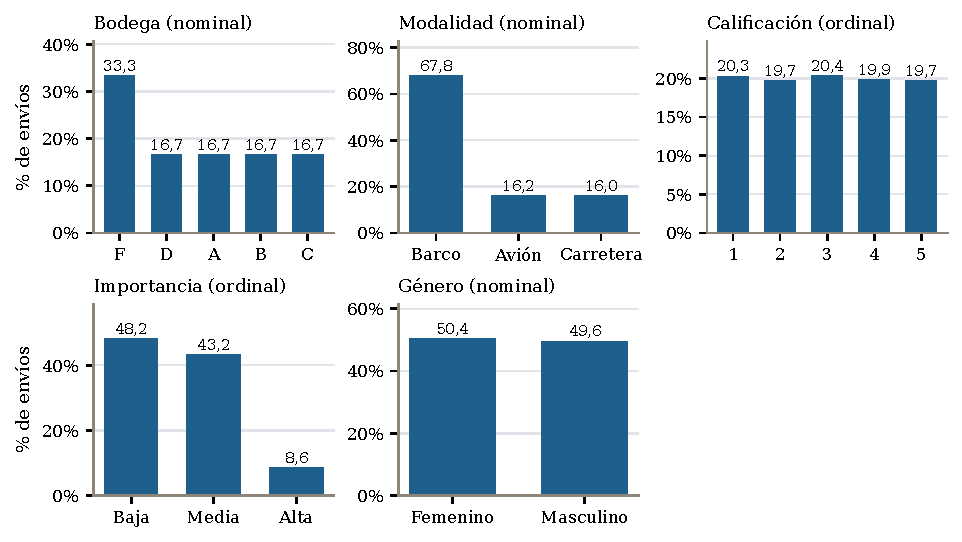
\includegraphics[width=0.88\linewidth,height=0.42\textheight,keepaspectratio]{../../outputs/figuras/fig_eda_3_cualitativas.pdf}
\caption{Frecuencias de variables cualitativas y ordinales.}\label{fig:anexo_cualitativas}
\end{figure}
La muestra está desbalanceada en dos variables: Barco concentra el 67,8\% de los envíos y la bodega F el 33,3\%, el doble que cada una de las otras cuatro (16,7\%). La importancia alta es la categoría más pequeña (8,6\%; 948 envíos), por lo que su tasa de atraso tiene el intervalo más ancho entre las tasas por categoría (Figura~\ref{fig:categorias}). Calificación (19,7--20,4\%) y género (49,6--50,4\%) están prácticamente equilibrados. Esta composición describe volumen, no riesgo: que Barco concentre la mayoría de los envíos no implica que se atrase más (T01).

\begin{figure}[H]\centering
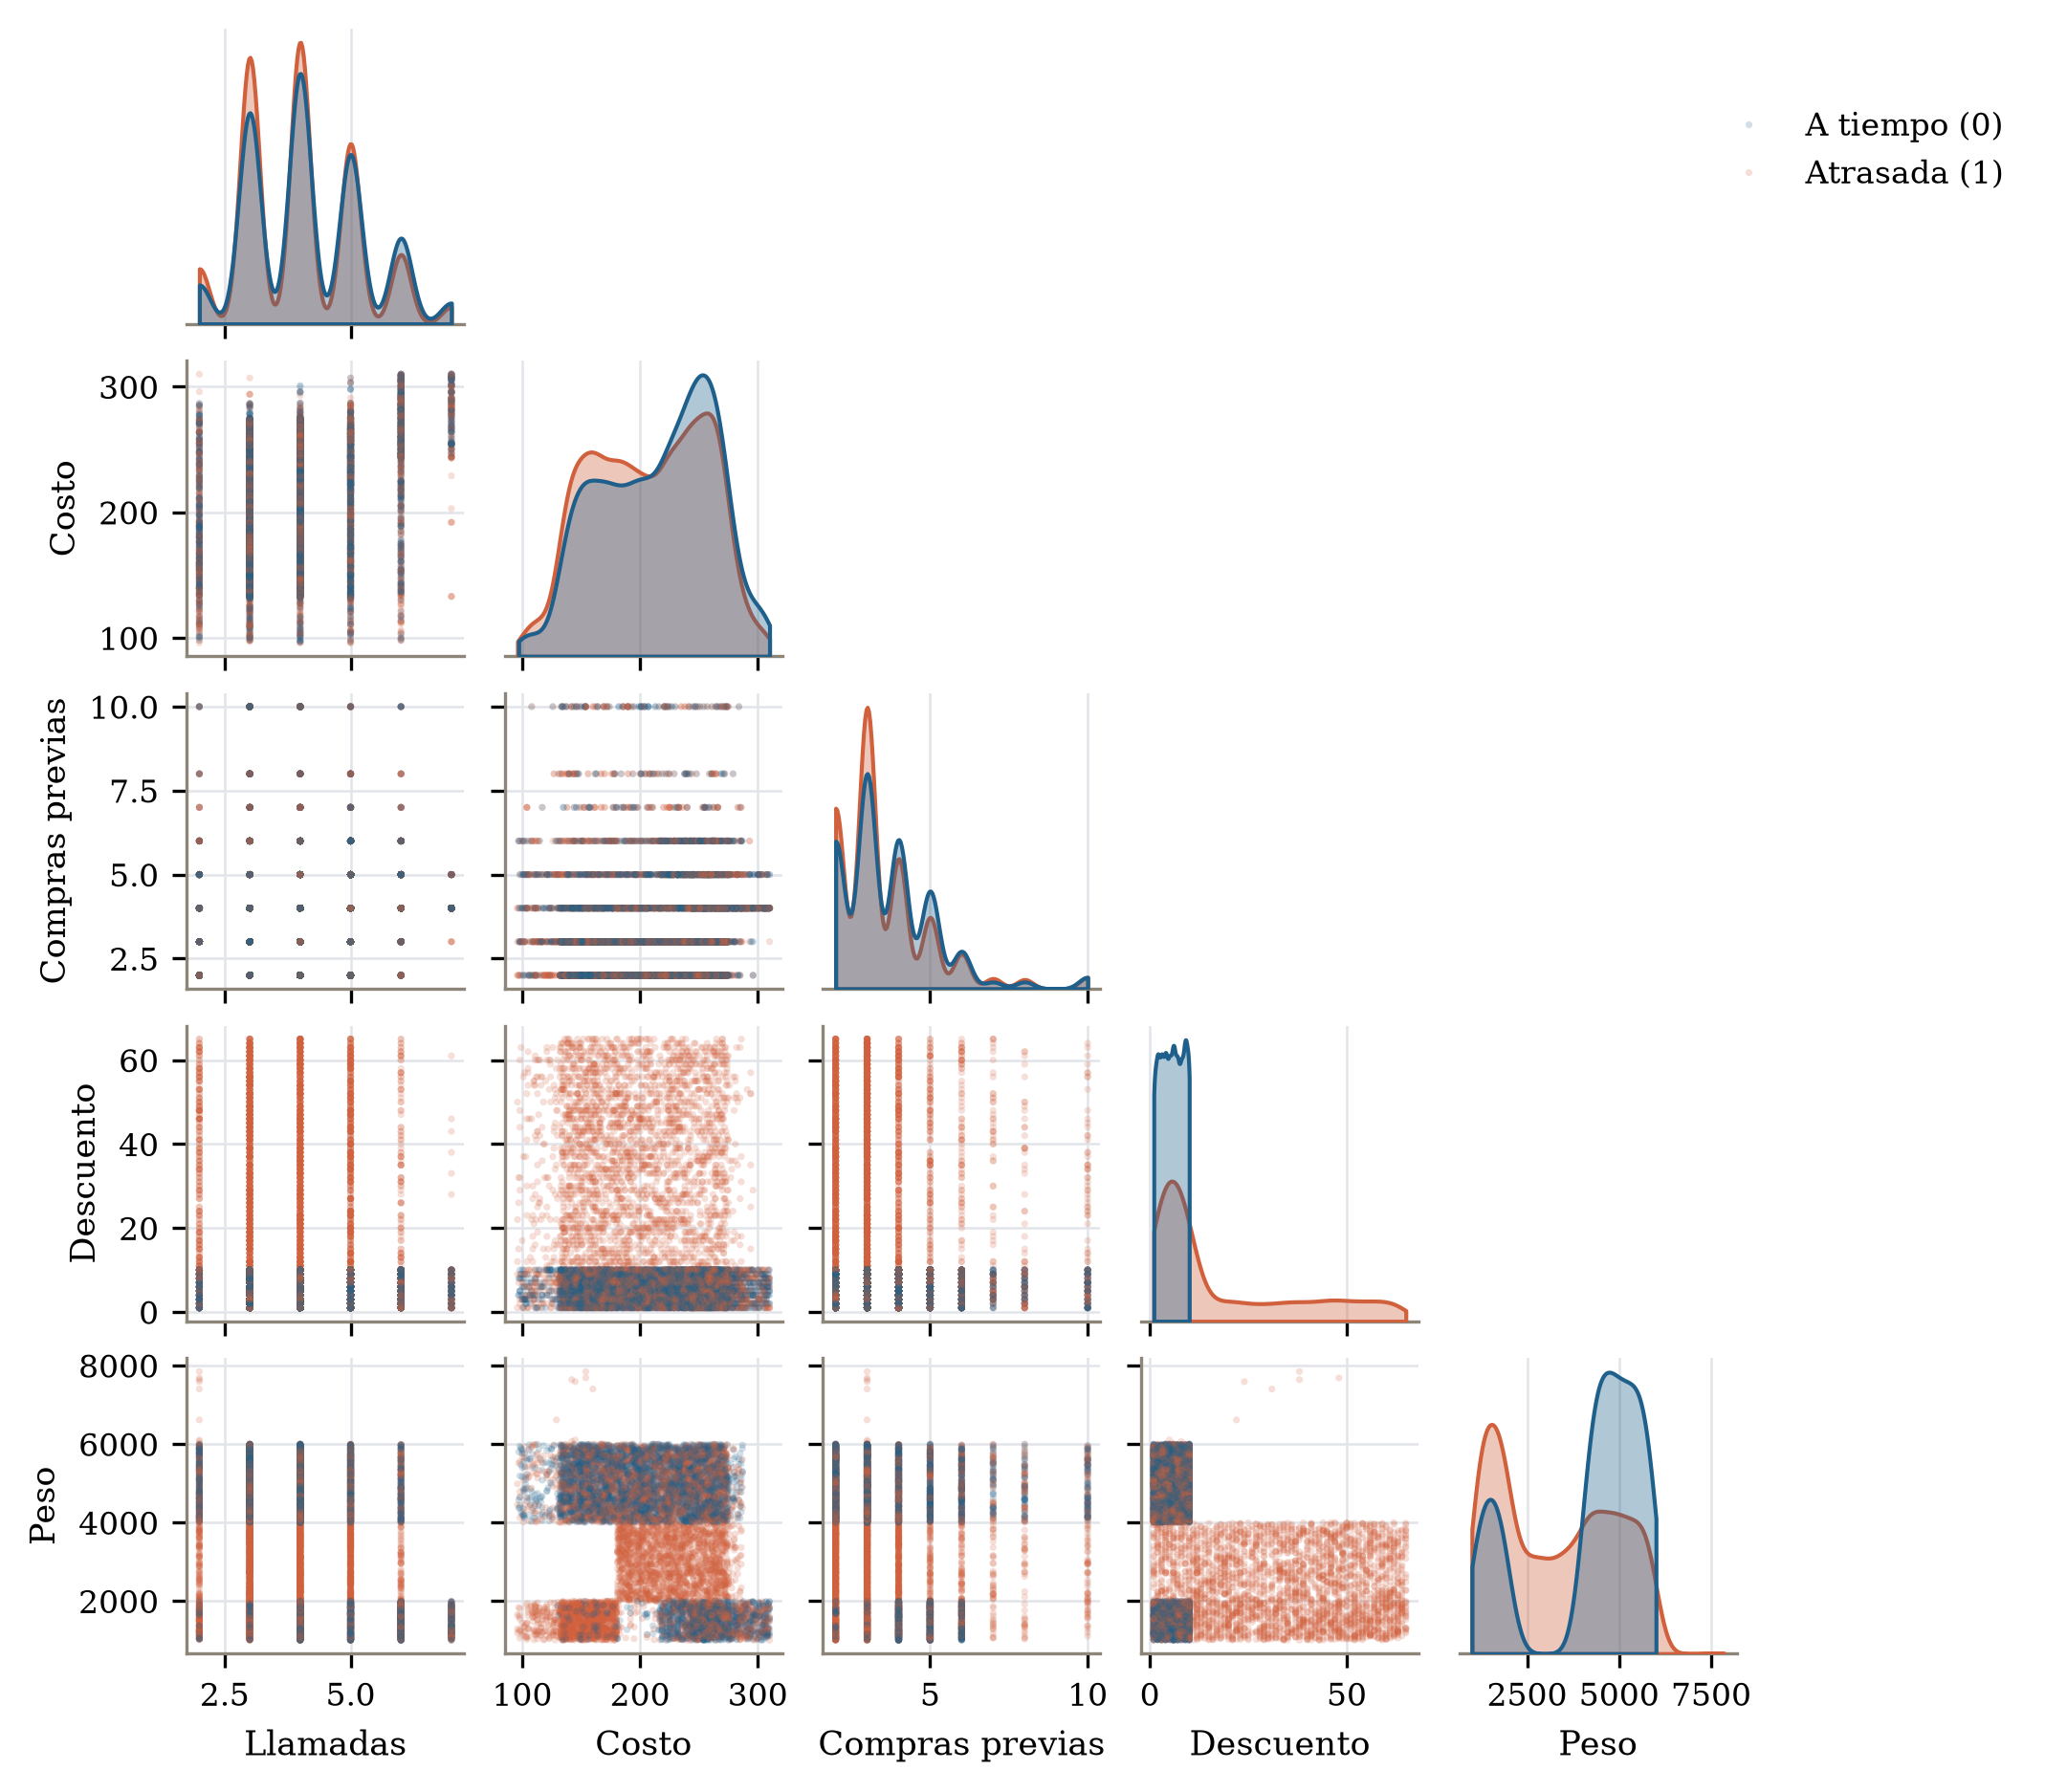
\includegraphics[width=0.88\linewidth,height=0.42\textheight,keepaspectratio]{../../outputs/figuras/fig_eda_4_pairplot.png}
\caption{Relaciones por pares entre variables cuantitativas.}\label{fig:anexo_pairplot}
\end{figure}
Las diagonales muestran que el peso y el descuento tienen distribuciones distintas según el resultado. En el peso, las entregas puntuales forman dos bloques separados: el 23,6\% pesa 2.000 g o menos y el 76,4\% entre 4.000 y 6.000 g, con una sola puntual en el tramo intermedio. Las atrasadas, en cambio, se reparten en los tres tramos (33,5\%, 27,2\% y 39,1\%) y son las únicas sobre 6.000 g. En el descuento, las puntuales se distribuyen de forma casi uniforme entre 1 y 10 (cerca del 10\% en cada valor) y ninguna supera ese valor; las atrasadas tienen el mismo bloque uniforme en el 59,7\% de los casos y, además, una cola plana entre 11 y 65 que reúne el 40,3\%. En llamadas, costo y compras previas, las densidades de ambos grupos casi se superponen. En los diagramas de dispersión, ningún envío de entre 4.000 y 6.000 g recibe un descuento mayor que 10, lo que explica la correlación negativa entre peso y descuento ($\rho=-0{,}32$); los demás pares no muestran una estructura marcada ($|\rho|\le0{,}29$).

\begin{figure}[H]\centering
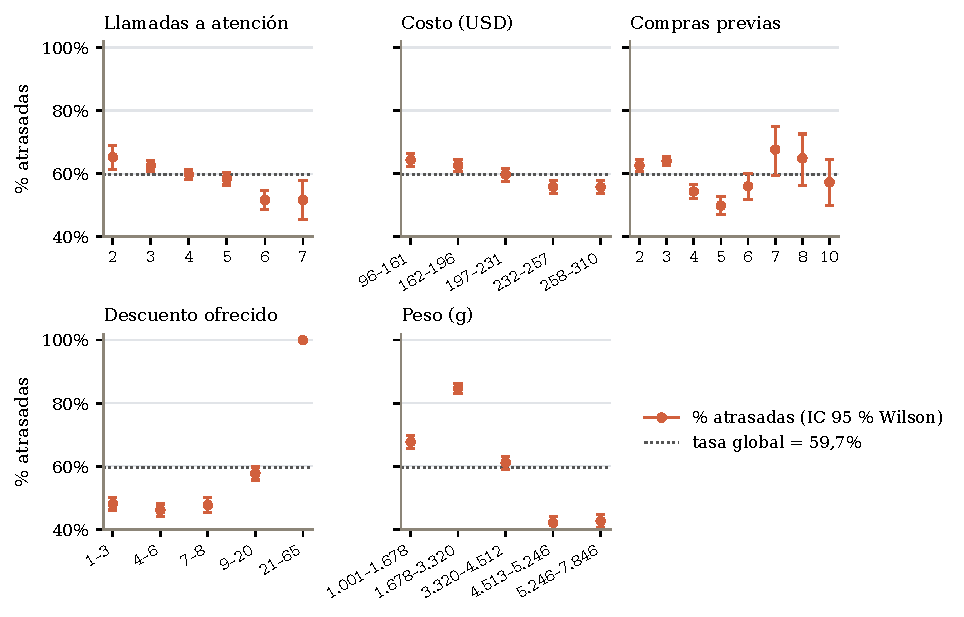
\includegraphics[width=0.88\linewidth,height=0.42\textheight,keepaspectratio]{../../outputs/figuras/fig_eda_6_dependiente_vs_cuantitativas.pdf}
\caption{Tasa de atraso por tramo de cada variable cuantitativa, con IC 95\% de Wilson.}\label{fig:anexo_cuant_obj}
\end{figure}
Solo el descuento y el peso producen cambios grandes en la tasa de atraso. Con descuentos de hasta 8, la tasa ronda el 46--48\%, por debajo de la global; en el quintil de 21 a 65 llega al 100\%. En el peso la relación no es monótona: la tasa sube de 67,7\% (1.001--1.678 g) a 84,7\% (1.678--3.320 g) y baja a cerca del 42\% sobre 4.512 g, por lo que la diferencia de medias de T02 resume mal este patrón. Llamadas y costo muestran un descenso gradual (de 65,2\% a 51,6\% y de 64,3\% a 55,7\%), y compras previas no tiene una tendencia clara; con 7, 8 y 10 compras, los intervalos son anchos porque hay pocos envíos.

\begin{figure}[H]\centering
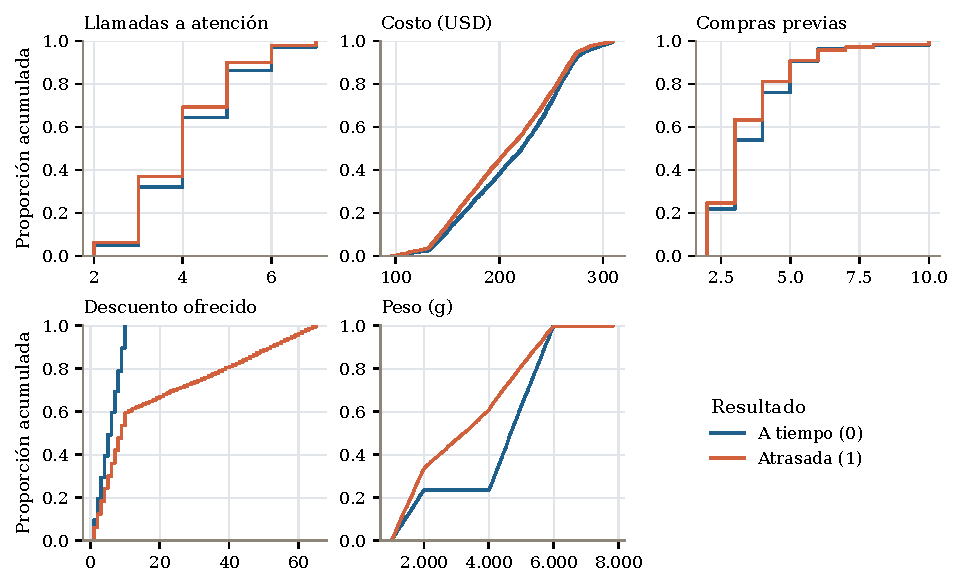
\includegraphics[width=0.88\linewidth,height=0.42\textheight,keepaspectratio]{../../outputs/figuras/fig_eda_6b_ecdf_por_resultado.pdf}
\caption{Funciones de distribución acumulada empírica por resultado.}\label{fig:anexo_ecdf}
\end{figure}
Las curvas muestran lo que el promedio oculta. En el peso, la ECDF de las entregas puntuales queda plana entre 2.000 y 4.000 g porque casi no hay envíos puntuales en ese tramo, mientras que la de las atrasadas crece en forma continua; las medianas son 4.674 g (puntuales) y 3.231 g (atrasadas). En el descuento, todas las puntuales tienen 10 o menos, frente a cerca del 60\% de las atrasadas. En llamadas, costo y compras previas, las curvas casi se superponen: las atrasadas tienden a valores algo menores (costo mediano de 209 frente a 222 USD), diferencias coherentes con efectos pequeños ($d_{av}$ entre $-0{,}11$ y $-0{,}15$).

\begin{figure}[H]\centering
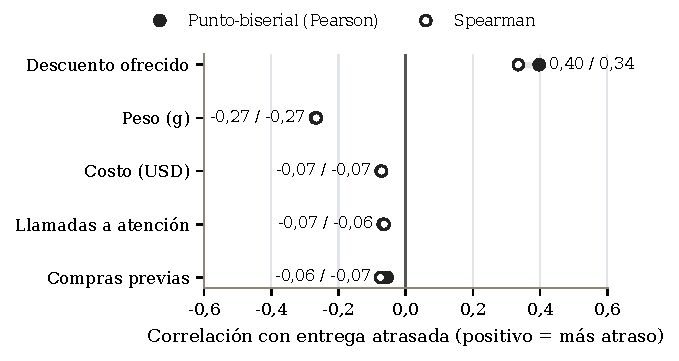
\includegraphics[width=0.88\linewidth,height=0.42\textheight,keepaspectratio]{../../outputs/figuras/fig_eda_7_correlacion_dependiente.pdf}
\caption{Correlación punto-biserial y de Spearman de cada variable cuantitativa con el atraso.}\label{fig:anexo_correlacion_obj}
\end{figure}
Solo el descuento ($r_{pb}=0{,}40$; $\rho=0{,}34$) y el peso ($-0{,}27$ con ambas medidas) tienen una asociación apreciable con el atraso; las otras tres variables no superan 0,08 en valor absoluto. En el descuento, la punto-biserial supera a la de Spearman porque los valores altos, todos atrasados, pesan más en una correlación lineal que en una de rangos. En el peso ambas coinciden, pero ninguna capta su relación no monótona (Figura~\ref{fig:anexo_cuant_obj}): una correlación de $-0{,}27$ subestima cuánto informa el peso sobre el atraso en el tramo de 2.000 a 4.000 g.

\begin{figure}[H]\centering
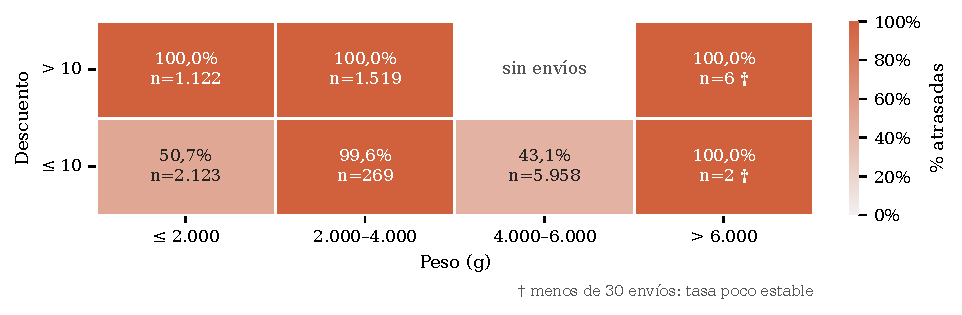
\includegraphics[width=0.88\linewidth,height=0.42\textheight,keepaspectratio]{../../outputs/figuras/fig_eda_9_descuento_x_peso.pdf}
\caption{Relación conjunta entre descuento, peso y atraso.}\label{fig:anexo_desc_peso}
\end{figure}
El cruce muestra dos condiciones que casi determinan el resultado: todos los envíos con descuento mayor que 10 llegaron atrasados, cualquiera sea su peso, y entre los envíos con descuento de 10 o menos, el tramo de 2.000 a 4.000 g tiene un 99,6\% de atraso. Fuera de esas condiciones la tasa queda por debajo de la global: 50,7\% bajo 2.000 g y 43,1\% entre 4.000 y 6.000 g, el segmento más grande (5.958 envíos). Así, la variación del resultado que queda por explicar se concentra en los envíos con descuento de 10 o menos fuera del tramo de 2.000--4.000 g. No hay envíos con descuento mayor que 10 entre 4.000 y 6.000 g, y sobre 6.000 g solo hay 8 envíos, por lo que esas celdas no permiten conclusiones.

\begin{figure}[H]\centering
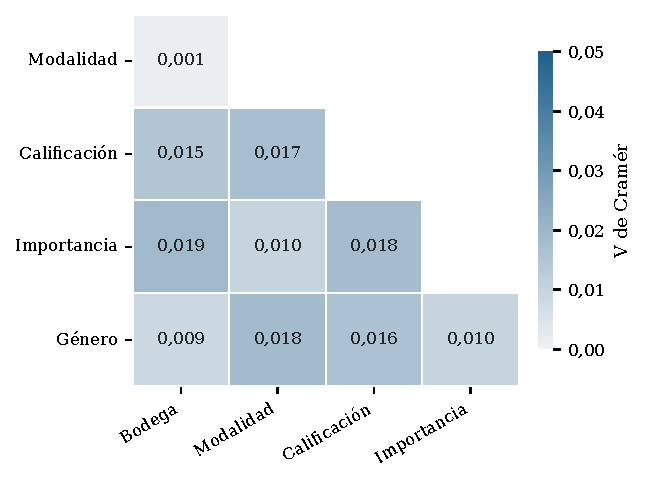
\includegraphics[width=0.88\linewidth,height=0.42\textheight,keepaspectratio]{../../outputs/figuras/fig_eda_10_cramer_cualitativas.pdf}
\caption{Magnitud de asociaciones categóricas mediante V de Cramér.}\label{fig:anexo_cramer}
\end{figure}
Todas las asociaciones entre variables cualitativas son prácticamente nulas: la mayor es $V=0{,}019$ (bodega e importancia) y la menor, $V=0{,}001$ (bodega y modalidad). Las variables no son redundantes, de modo que sus tasas de atraso por categoría (Figura~\ref{fig:categorias}) pueden leerse una por una: el exceso de atraso de la importancia alta no puede atribuirse a que se concentre en alguna bodega o modalidad.

\begin{figure}[H]\centering
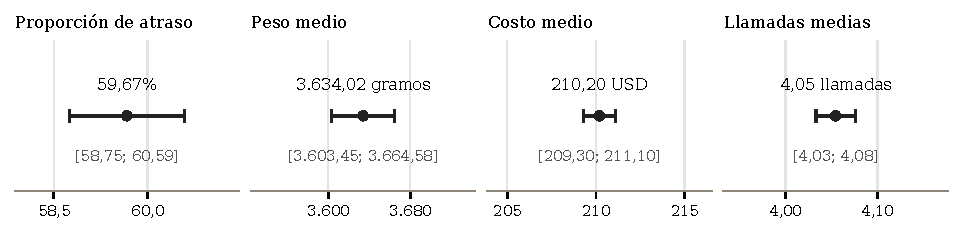
\includegraphics[width=0.88\linewidth,height=0.42\textheight,keepaspectratio]{../../outputs/figuras/fig_inf_1_intervalos.pdf}
\caption{Visualización de estimaciones e intervalos de confianza.}\label{fig:anexo_intervalos}
\end{figure}
En una escala común de $\pm3\%$ alrededor de cada estimación, los cuatro intervalos son estrechos: el más ancho, el de la proporción de atraso ([58,75\%; 60,58\%]), equivale al 3,1\% del valor estimado, y el más angosto, el del costo, al 0,85\%. Con $n=10\,999$, la incertidumbre de muestreo es pequeña frente a otras fuentes de error que estos intervalos no reflejan, como la forma en que se seleccionaron los registros.

\begin{figure}[H]\centering
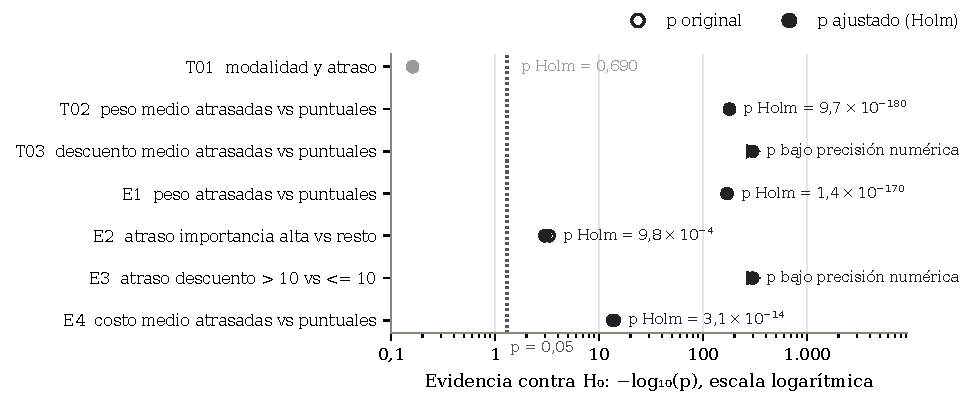
\includegraphics[width=0.88\linewidth,height=0.42\textheight,keepaspectratio]{../../outputs/figuras/fig_inf_2_holm.pdf}
\caption{Resultados de las pruebas y ajuste por multiplicidad de Holm.}\label{fig:anexo_holm}
\end{figure}
Seis de los siete contrastes rechazan $H_0$ antes y después del ajuste, que no cambia ninguna decisión. El caso más cercano al umbral es E2 (importancia alta), con un $p$ ajustado de 0,001, unas 50 veces menor que 0,05; T01 (modalidad) queda lejos de él ($p=0{,}69$). En T03 y E3 el $p$ es tan pequeño que se informa como menor que $10^{-300}$. Que la evidencia sea fuerte no significa que los efectos sean grandes: E4 es significativa con un efecto muy pequeño ($d_{av}=-0{,}15$).

\clearpage
\section{Técnicas estadísticas empleadas y justificación}\label{sec:anexo_tecnicas}
\small
Cada técnica se documenta con cinco campos: \textbf{qué es}, \textbf{fórmula}, \textbf{por qué se eligió en este caso} (con las cifras de estos datos), \textbf{supuestos y precauciones} e \textbf{implementación}. Notación: subíndice $a$ = entregas atrasadas ($n_a=6\,563$), $p$ = puntuales ($n_p=4\,436$), $n=10\,999$; $z=z_{0{,}975}=1{,}95996$.

\subsection{Estadística descriptiva}

\subsubsection{Media, mediana, desviación estándar, cuartiles e IQR}
\textbf{Qué es.} Medidas de centro (media, mediana) y de dispersión (desviación estándar, cuartiles y rango intercuartílico) de cada variable cuantitativa.

\textbf{Fórmula.}
\[
\bar x=\frac1n\sum_{i=1}^{n}x_i,\qquad
s=\sqrt{\frac{1}{n-1}\sum_{i=1}^{n}(x_i-\bar x)^2},\qquad
\mathrm{IQR}=Q_3-Q_1,
\]
donde $Q_1$, la mediana ($Q_2$) y $Q_3$ son los cuantiles 0,25, 0,50 y 0,75, calculados por interpolación lineal entre observaciones ordenadas.

\textbf{Por qué aquí.} La media y la desviación estándar son la base de los intervalos y de la prueba de Welch. Como varias variables son asimétricas, se reportan además la mediana y el IQR, que no dependen de la magnitud de los valores extremos: en el descuento la media (13,37) casi duplica la mediana (7). En el peso, bimodal, ni la media (3.634,02 g) ni la mediana (4.149 g) describen por sí solas a un envío típico, por lo que se complementan con histogramas.

\textbf{Supuestos y precauciones.} La media y la desviación estándar son sensibles a valores extremos; la mediana y el IQR son robustos. La desviación estándar usa $n-1$ para estimar sin sesgo la varianza poblacional.

\textbf{Implementación.} \texttt{DataFrame.describe()}; \texttt{std(ddof=1)}; \texttt{quantile()}.

\subsubsection{Regla de 1,5·IQR para valores extremos}
\textbf{Qué es.} Criterio de Tukey (1977) para señalar observaciones alejadas del centro de la distribución.

\textbf{Fórmula.} Una observación es extrema si
\[
x_i<Q_1-1{,}5\,\mathrm{IQR}\quad\text{o}\quad x_i>Q_3+1{,}5\,\mathrm{IQR}.
\]

\textbf{Por qué aquí.} No supone normalidad y usa cuartiles, que no se ven afectados por los propios extremos. Identifica 1.003 valores altos en compras previas y 2.209 en descuento; se conservan porque son valores válidos, no errores de registro.

\textbf{Supuestos y precauciones.} En distribuciones asimétricas la regla marca como ``extrema'' gran parte de la cola sin que esos valores sean anómalos: en el descuento señala el 20,1\% de los registros. Por eso se usa para describir, no para eliminar datos.

\textbf{Implementación.} Cálculo directo con \texttt{quantile([0.25, 0.75])}.

\subsubsection{Asimetría y curtosis en exceso ajustadas}
\textbf{Qué es.} Medidas de forma basadas en el tercer y el cuarto momento: la asimetría ($G_1$) indica hacia qué lado se extiende la cola; la curtosis en exceso ($G_2$), el peso de las colas respecto de la normal.

\textbf{Fórmula.} Con los momentos centrales $m_k=\frac1n\sum(x_i-\bar x)^k$:
\[
G_1=\frac{\sqrt{n(n-1)}}{n-2}\,\frac{m_3}{m_2^{3/2}},\qquad
G_2=\frac{n-1}{(n-2)(n-3)}\left[(n+1)\left(\frac{m_4}{m_2^{2}}-3\right)+6\right].
\]
$G_2$ sigue la definición de Fisher (curtosis de Pearson $-\,3$), de modo que una normal tiene $G_1=G_2=0$ (Joanes y Gill, 1998).

\textbf{Por qué aquí.} Cuantifica lo que muestran los histogramas y orienta qué resúmenes usar. Descuento ($G_1=1{,}80$; $G_2=2{,}00$) y compras previas ($G_1=1{,}68$; $G_2=4{,}01$) tienen colas derechas pesadas, por lo que la mediana es más representativa que la media. El peso tiene $G_2=-1{,}45$, reflejo de su bimodalidad.

\textbf{Supuestos y precauciones.} No son pruebas de normalidad. Al elevar desviaciones a la tercera y cuarta potencia, los pocos valores altos dominan ambas medidas. Un $G_2$ negativo en una variable bimodal no significa colas ``livianas'' en el sentido habitual.

\textbf{Implementación.} \texttt{scipy.stats.skew(bias=False)}; \texttt{scipy.stats.kurtosis(fisher=True, bias=False)}.

\subsubsection{Función de distribución acumulada empírica (ECDF)}
\textbf{Qué es.} Para cada valor $x$, la proporción de observaciones del grupo que no lo superan.

\textbf{Fórmula.}
\[
\hat F_n(x)=\frac1n\sum_{i=1}^{n}\mathbf 1(x_i\le x).
\]

\textbf{Por qué aquí.} Compara la distribución completa de atrasadas y puntuales sin elegir intervalos de histograma ni ocultar valores. En el descuento muestra lo que un diagrama de caja oculta: la ECDF de las puntuales llega al 100\% en 10, mientras que cerca del 40\% de las atrasadas supera ese valor.

\textbf{Supuestos y precauciones.} Es descriptiva; la diferencia entre curvas no se contrasta formalmente con esta técnica.

\textbf{Implementación.} \texttt{seaborn.ecdfplot}.

\subsubsection{Frecuencias y tasas por categoría}
\textbf{Qué es.} Conteo y porcentaje de cada categoría, y proporción de entregas atrasadas dentro de cada una.

\textbf{Fórmula.} Para la categoría $k$, con $x_k$ atrasos entre $n_k$ envíos: $\hat p_k=x_k/n_k$.

\textbf{Por qué aquí.} Es la única descripción válida para variables nominales (bodega, modalidad, género), y para las ordinales (calificación, importancia) se presenta respetando su orden. La tasa por categoría permite comparar cada grupo con la tasa global (59,67\%).

\textbf{Supuestos y precauciones.} La composición de la muestra (cuántos envíos hay por categoría) no es la tasa de atraso. Cada tasa se acompaña de su IC de Wilson (B.3.2).

\textbf{Implementación.} \texttt{value\_counts()}; \texttt{groupby().mean()}; \texttt{pandas.crosstab}.

\subsection{Medidas de asociación}

\subsubsection{Correlación de Spearman}
\textbf{Qué es.} Correlación de Pearson calculada sobre los rangos de las observaciones (Spearman, 1904). Mide asociación monótona, sea o no lineal, entre $-1$ y $1$.

\textbf{Fórmula.} Con $R_i$ y $S_i$ los rangos de $x_i$ e $y_i$ (rangos promedio en caso de empates):
\[
\rho_s=\frac{\sum_i(R_i-\bar R)(S_i-\bar S)}{\sqrt{\sum_i(R_i-\bar R)^2\sum_i(S_i-\bar S)^2}}.
\]
La fórmula abreviada $1-6\sum d_i^2/[n(n^2-1)]$ solo es exacta sin empates, lo que no ocurre en estos datos.

\textbf{Por qué aquí.} Las variables no cumplen las condiciones en que Pearson es adecuado: descuento y compras previas son muy asimétricas, el peso es bimodal y llamadas y compras previas son conteos con muchos empates. Al usar rangos, ningún valor extremo domina el coeficiente. La mayor asociación entre predictoras es peso--descuento ($\rho_s=-0{,}316$).

\textbf{Supuestos y precauciones.} No detecta relaciones no monótonas: la relación del peso con el atraso, alta en 2.000--4.000 g y baja en los extremos, no se refleja bien en un solo coeficiente. No implica causalidad.

\textbf{Implementación.} \texttt{DataFrame.corr(method='spearman')}; \texttt{scipy.stats.spearmanr}.

\subsubsection{Correlación punto-biserial}
\textbf{Qué es.} Correlación de Pearson entre una variable cuantitativa y una binaria codificada 0/1.

\textbf{Fórmula.} Con $s_n$ la desviación estándar de todas las observaciones (denominador $n$):
\[
r_{pb}=\frac{\bar x_a-\bar x_p}{s_n}\sqrt{\frac{n_a\,n_p}{n^2}}.
\]

\textbf{Por qué aquí.} El resultado es binario (1 = atrasada), por lo que la correlación de Pearson con cada predictora es la punto-biserial. Se presenta junto a Spearman para comprobar que el signo y el orden de las asociaciones no dependen del método: descuento $r_{pb}=0{,}397$ ($\rho_s=0{,}335$) y peso $r_{pb}=-0{,}269$ ($\rho_s=-0{,}266$).

\textbf{Supuestos y precauciones.} Como toda correlación de Pearson, es sensible a valores extremos y solo capta la parte lineal de la relación. Su valor máximo posible depende de la proporción de unos.

\textbf{Implementación.} \texttt{scipy.stats.pointbiserialr}.

\subsubsection{V de Cramér}
\textbf{Qué es.} Medida de la intensidad de asociación entre dos variables categóricas, entre 0 (independencia en la muestra) y 1 (asociación perfecta) (Cramér, 1946).

\textbf{Fórmula.} Para una tabla de $f$ filas y $c$ columnas:
\[
V=\sqrt{\frac{\chi^2}{n\,(\min(f,c)-1)}}.
\]

\textbf{Por qué aquí.} Con $n=10\,999$, la prueba $\chi^2$ detecta asociaciones mínimas; $V$ elimina el efecto del tamaño muestral y expresa la magnitud. Frente al atraso, la mayor es la de la importancia ($V=0{,}033$) y la de modalidad es $V=0{,}0082$; entre las cualitativas ninguna supera 0,019, por lo que no son redundantes entre sí.

\textbf{Supuestos y precauciones.} No indica dirección ni qué categoría difiere (para eso se usan las tasas por categoría). Ignora el orden de las variables ordinales y tiene un leve sesgo positivo en muestras pequeñas, despreciable aquí.

\textbf{Implementación.} \texttt{scipy.stats.contingency.association(method='cramer')}.

\subsection{Estimación por intervalos}

\subsubsection{Intervalo \texorpdfstring{$t$}{t} de Student para una media}
\textbf{Qué es.} Intervalo de confianza al 95\% para la media poblacional cuando la desviación estándar poblacional es desconocida.

\textbf{Fórmula.}
\[
\bar x\pm t_{0{,}975;\,n-1}\,\frac{s}{\sqrt n},\qquad t_{0{,}975;\,10\,998}=1{,}96018.
\]

\textbf{Por qué aquí.} Se estima $\sigma$ con $s$, y la distribución $t$ incorpora esa incertidumbre. Con $n=10\,999$ coincide con la aproximación normal del TCL ($z=1{,}95996$) hasta el segundo decimal. El TCL respalda la normalidad aproximada de la media de peso (bimodal), costo y llamadas (discreta), cuyas asimetrías son bajas ($|G_1|\le0{,}39$). No se estima la media del descuento, cuya unidad no está documentada.

\textbf{Supuestos y precauciones.} Independencia entre envíos, no verificable con estas columnas. El intervalo es individual, sin ajuste por comparaciones múltiples.

\textbf{Implementación.} \texttt{scipy.stats.t.ppf}; \texttt{std(ddof=1)}.

\subsubsection{Intervalo de Wilson para una proporción}
\textbf{Qué es.} Intervalo de confianza para una proporción binomial obtenido invirtiendo la prueba $z$ de puntuación (\emph{score}) (Wilson, 1927).

\textbf{Fórmula.}
\[
\frac{\hat p+\dfrac{z^2}{2n}\pm z\sqrt{\dfrac{\hat p(1-\hat p)}{n}+\dfrac{z^2}{4n^2}}}{1+\dfrac{z^2}{n}}.
\]

\textbf{Por qué aquí.} El intervalo de Wald ($\hat p\pm z\sqrt{\hat p(1-\hat p)/n}$) tiene una cobertura irregular, por debajo del 95\% nominal incluso con $n$ moderado, y se degenera cuando $\hat p=0$ o $1$ (Brown et al., 2001). Aquí se estiman tasas en categorías desde 948 envíos y en grupos con 100\% de atraso: con descuento mayor que 10, Wilson da [99,86\%; 100\%] en vez del intervalo de ancho cero de Wald. Para la tasa global da [58,75\%; 60,58\%].

\textbf{Supuestos y precauciones.} Independencia entre envíos. Los intervalos por categoría son individuales: que se superpongan o no, no reemplaza una prueba de hipótesis.

\textbf{Implementación.} \texttt{proportion\_confint(method='wilson')}, de \texttt{statsmodels.stats.proportion}.

\subsection{Pruebas de hipótesis}

\subsubsection{Prueba \texorpdfstring{$\chi^2$}{chi-cuadrado} de independencia (T01)}
\textbf{Qué es.} Contrasta si dos variables categóricas son independientes, comparando las frecuencias observadas con las esperadas bajo independencia.

\textbf{Fórmula.}
\[
\chi^2=\sum_{i=1}^{f}\sum_{j=1}^{c}\frac{(O_{ij}-E_{ij})^2}{E_{ij}},\qquad
E_{ij}=\frac{(\text{total fila } i)(\text{total columna } j)}{n},\qquad
\text{gl}=(f-1)(c-1).
\]

\textbf{Por qué aquí.} Modalidad (3 categorías) y resultado (2) son categóricas, y la pregunta es si la tasa de atraso depende de la modalidad. La aproximación $\chi^2$ requiere frecuencias esperadas suficientes: la mínima es 709,82, muy por encima del umbral habitual de 5. Resultado: $\chi^2(2)=0{,}7434$, $p=0{,}690$. Con 2 grados de libertad no se aplica la corrección de continuidad de Yates.

\textbf{Supuestos y precauciones.} Independencia entre envíos. La prueba no mide la magnitud de la asociación (para eso, $V$ de Cramér), y no rechazar $H_0$ no demuestra independencia.

\textbf{Implementación.} \texttt{scipy.stats.chi2\_contingency}.

\subsubsection{Prueba \texorpdfstring{$t$}{t} de Welch (T02, T03, E4)}
\textbf{Qué es.} Contrasta si dos medias poblacionales difieren, sin suponer varianzas iguales entre los grupos (Welch, 1947).

\textbf{Fórmula.}
\[
t=\frac{\bar x_a-\bar x_p}{\sqrt{s_a^2/n_a+s_p^2/n_p}},\qquad
\nu=\frac{\left(s_a^2/n_a+s_p^2/n_p\right)^2}{\dfrac{(s_a^2/n_a)^2}{n_a-1}+\dfrac{(s_p^2/n_p)^2}{n_p-1}},
\]
con IC al 95\% para la diferencia: $(\bar x_a-\bar x_p)\pm t_{0{,}975;\,\nu}\sqrt{s_a^2/n_a+s_p^2/n_p}$.

\textbf{Por qué aquí.} Los grupos tienen tamaños distintos y, en el descuento, varianzas muy distintas (desviaciones estándar de 19,11 y 2,88). La $t$ clásica supone varianzas iguales y en ese escenario distorsiona la tasa de error tipo I; Welch mantiene el nivel nominal. Cuando las varianzas son similares, como en peso (1.576 y 1.574 g) y costo, coincide con la $t$ clásica, por lo que usarlo siempre no tiene costo.

\textbf{Supuestos y precauciones.} Independencia entre envíos. La normalidad aproximada de las medias se apoya en el TCL por el tamaño de los grupos, pese a la bimodalidad del peso; E1 verifica que la conclusión de T02 no dependa de ese supuesto.

\textbf{Implementación.} \texttt{scipy.stats.ttest\_ind(equal\_var=False)}; \texttt{confidence\_interval(0.95)}.

\subsubsection{Prueba de Mann--Whitney (E1)}
\textbf{Qué es.} Prueba no paramétrica que compara dos grupos a partir de los rangos de las observaciones combinadas (Mann y Whitney, 1947).

\textbf{Fórmula.} Con $R_a$ la suma de rangos de las atrasadas en la muestra combinada:
\[
U_a=R_a-\frac{n_a(n_a+1)}{2},\qquad
z=\frac{U_a-n_an_p/2\mp0{,}5}{\sigma_U},\qquad
\sigma_U^2=\frac{n_an_p}{12}\left[(n+1)-\frac{\sum_k(t_k^3-t_k)}{n(n-1)}\right],
\]
donde $t_k$ es el número de observaciones empatadas en el valor $k$ y $\mp0{,}5$ es la corrección de continuidad.

\textbf{Por qué aquí.} Complementa T02 sin depender de la normalidad ni de que la media represente bien a una variable bimodal como el peso. Al usar rangos, ninguna observación influye por su magnitud. Resultado: $U=10\,000\,332{,}5$, $p=3{,}40\times10^{-171}$; la conclusión coincide con T02.

\textbf{Supuestos y precauciones.} Independencia entre envíos. Contrasta si un grupo tiende a tomar valores mayores que el otro, es decir, $P(X_a>X_p)\ne1/2$; solo equivale a comparar medianas si ambas distribuciones tienen la misma forma, lo que no ocurre con el peso.

\textbf{Implementación.} \texttt{scipy.stats.mannwhitneyu(method='asymptotic', use\_continuity=True)}.

\subsubsection{Prueba \texorpdfstring{$z$}{z} de dos proporciones e intervalo de Newcombe (E2, E3)}
\textbf{Qué es.} La prueba $z$ contrasta si dos proporciones poblacionales son iguales; el intervalo de Newcombe estima su diferencia (Newcombe, 1998).

\textbf{Fórmula.} Con $\bar p=(x_1+x_0)/(n_1+n_0)$ la proporción combinada bajo $H_0$:
\[
z=\frac{\hat p_1-\hat p_0}{\sqrt{\bar p(1-\bar p)\left(\frac1{n_1}+\frac1{n_0}\right)}}.
\]
Con $(l_1,u_1)$ y $(l_0,u_0)$ los intervalos de Wilson de cada grupo y $\hat\Delta=\hat p_1-\hat p_0$, el IC de Newcombe es
\[
\left[\hat\Delta-\sqrt{(\hat p_1-l_1)^2+(u_0-\hat p_0)^2}\,;\ \hat\Delta+\sqrt{(u_1-\hat p_1)^2+(\hat p_0-l_0)^2}\right].
\]

\textbf{Por qué aquí.} El resultado es binario y se comparan dos grupos: importancia alta frente al resto (E2) y descuento mayor que 10 frente al resto (E3). La proporción combinada es la correcta bajo $H_0$, y la prueba equivale a la $\chi^2$ de una tabla $2\times2$ ($z^2=\chi^2$). Para el intervalo se usa Newcombe y no Wald porque en E3 un grupo tiene proporción 1: Wald le asignaría varianza cero, mientras que Newcombe hereda el comportamiento de Wilson. Resultados: E2, diferencia de 5,81 pp, IC [2,57; 8,93] pp, $z=3{,}486$; E3, diferencia de 53,11 pp, IC [52,03; 54,18] pp, $z=48{,}54$.

\textbf{Supuestos y precauciones.} Independencia entre envíos. El umbral de 10 del descuento proviene del EDA, por lo que E3 es exploratorio y requiere validación independiente.

{\sloppy \textbf{Implementación.} Prueba $z$ calculada directamente con \texttt{scipy.stats.norm.sf}; IC con \texttt{confint\_proportions\_2indep(method='newcomb')}, de \texttt{statsmodels.stats.proportion}.\par}

\subsection{Tamaños de efecto}

\subsubsection{\texorpdfstring{$d_{av}$}{d\_av}: d de Cohen con desviación estándar promedio}
\textbf{Qué es.} Diferencia de medias expresada en desviaciones estándar. Es una variante de la d de Cohen, también llamada $d'$ o $d^*$ (Cohen, 1988; Delacre et al., 2021).

\textbf{Fórmula.}
\[
d_{av}=\frac{\bar x_a-\bar x_p}{\sqrt{\left(s_a^2+s_p^2\right)/2}}.
\]
A diferencia de la d clásica, cuyo denominador pondera las varianzas por $n-1$, aquí ambos grupos pesan igual.

\textbf{Por qué aquí.} Con $n=10\,999$ casi cualquier diferencia es significativa, por lo que se necesita una medida de magnitud. Se eligió esta variante porque no supone varianzas iguales ni depende de cuál grupo es más grande, en coherencia con la prueba de Welch. Resultados: peso $-0{,}569$, descuento $0{,}960$ y costo $-0{,}150$. Como referencia orientativa, Cohen (1988) sugiere 0,2, 0,5 y 0,8 para efectos pequeños, medianos y grandes.

\textbf{Supuestos y precauciones.} Cuando las varianzas difieren mucho, el valor depende de cómo se combinan: en el descuento, la d clásica daría 0,882 en vez de 0,960, con la misma interpretación (efecto grande). Los umbrales de Cohen no reemplazan un criterio de relevancia operacional.

\textbf{Implementación.} Cálculo directo; columna \texttt{d\_av} de las tablas exportadas.

\subsubsection{Correlación biserial de rangos (efecto de E1)}
\textbf{Qué es.} Tamaño de efecto asociado a Mann--Whitney, entre $-1$ y $1$ (Kerby, 2014).

\textbf{Fórmula.}
\[
r_{rb}=\frac{2U_a}{n_a\,n_p}-1=P(X_a>X_p)-P(X_a<X_p).
\]

\textbf{Por qué aquí.} Es la medida de magnitud coherente con una prueba de rangos y se interpreta directamente como probabilidad. Con $r_{rb}=-0{,}313$, al comparar un envío atrasado con uno puntual elegidos al azar, es más probable que el puntual pese más.

\textbf{Supuestos y precauciones.} Resume el desplazamiento entre las distribuciones, no la diferencia de medianas.

\textbf{Implementación.} Cálculo directo a partir del estadístico $U$ de \texttt{mannwhitneyu}.

\subsubsection{Diferencia de proporciones y riesgo relativo (E2, E3)}
\textbf{Qué es.} Comparación absoluta y relativa de dos tasas de atraso.

\textbf{Fórmula.}
\[
\hat\Delta=\hat p_1-\hat p_0\ \text{(puntos porcentuales)},\qquad
\widehat{RR}=\frac{\hat p_1}{\hat p_0}.
\]

\textbf{Por qué aquí.} La diferencia indica cuántos puntos porcentuales cambia la tasa y el riesgo relativo, cuántas veces es mayor. En E3, la tasa con descuento mayor que 10 es 53,11 pp mayor y 2,13 veces la del resto.

\textbf{Supuestos y precauciones.} El riesgo relativo se reporta de forma descriptiva, sin intervalo de confianza.

\textbf{Implementación.} Cálculo directo.

\subsection{Comparaciones múltiples}

\subsubsection{Corrección de Holm}
\textbf{Qué es.} Procedimiento secuencial que controla la probabilidad de cometer al menos un error tipo I en una familia de $m$ pruebas (\emph{familywise error rate}) (Holm, 1979).

\textbf{Fórmula.} Se ordenan los valores $p$ de menor a mayor, $p_{(1)}\le\dots\le p_{(m)}$, y se rechaza $H_{(i)}$ mientras $p_{(i)}\le\alpha/(m-i+1)$, deteniéndose en la primera que no cumple. Los valores $p$ ajustados son
\[
\tilde p_{(i)}=\max_{j\le i}\ \min\left\{1,\ (m-j+1)\,p_{(j)}\right\}.
\]

\textbf{Por qué aquí.} Se reportan siete contrastes ($m=7$) y, sin ajuste, la probabilidad de algún falso positivo supera el 5\%. Holm controla ese error con cualquier estructura de dependencia entre las pruebas y siempre rechaza al menos lo mismo que Bonferroni, por lo que es más potente. Ninguna decisión cambia tras el ajuste.

\textbf{Supuestos y precauciones.} Solo corrige por las siete pruebas de la familia: no valida umbrales derivados del EDA, como el de descuento mayor que 10.

\textbf{Implementación.} \texttt{statsmodels.stats.multitest.multipletests(method='holm')}.


\paragraph{Criterios transversales de interpretación.}
En todas las técnicas se distingue magnitud del efecto, significancia estadística y utilidad operacional. La muestra no documenta marco de selección, fechas o identificación de clientes; por ello, independencia y representatividad no quedan verificadas. El descuento podría ser posterior al atraso, lo cual impediría utilizarlo como predictor prospectivo sin establecer su temporalidad.

\paragraph{Trazabilidad.}
Las implementaciones y tablas se encuentran en el notebook y en \texttt{sumativa\_1/outputs/tablas/}; las figuras proceden de \texttt{sumativa\_1/outputs/figuras/}. El anexo conserva los nombres originales de archivo y remite al código reproducible del proyecto.

\end{document}